\documentclass[10pt,twocolumn,letterpaper]{article}

% My own stuff
\usepackage{booktabs}
% \usepackage{caption}
% \captionsetup[table]{skip=8pt}   % Only affects tables
\usepackage{stfloats}  % Add this to the preamble
\usepackage{float}
\usepackage[T1]{fontenc}
\usepackage[utf8]{inputenc}  % Ensure UTF-8 encoding


\usepackage{cvpr}
\usepackage{times}
\usepackage{epsfig}
\usepackage{graphicx}
\usepackage{amsmath}
\usepackage{amssymb}

% Include other packages here, before hyperref.

% If you comment hyperref and then uncomment it, you should delete
% egpaper.aux before re-running latex.  (Or just hit 'q' on the first latex
% run, let it finish, and you should be clear).
\usepackage[breaklinks=true,bookmarks=false]{hyperref}

\cvprfinalcopy % *** Uncomment this line for the final submission

\def\cvprPaperID{****} % *** Enter the CVPR Paper ID here
\def\httilde{\mbox{\tt\raisebox{-.5ex}{\symbol{126}}}}

% Pages are numbered in submission mode, and unnumbered in camera-ready
%\ifcvprfinal\pagestyle{empty}\fi
\setcounter{page}{1}
\begin{document}

%%%%%%%%% TITLE
\title{ECDO Datengetriebenes Primer Teil 1/2: Aktuelles Verständnis der Exothermen Kern-Mantel-Entkopplung Dzhanibekov-Oszillation (ECDO) „Erdumkippen“-Theorie}

\author{Junho\\
Website: \href{https://sovrynn.github.io}{sovrynn.github.io}\\
ECDO Forschungsrepo: \href{https://github.com/sovrynn/ecdo}{github.com/sovrynn/ecdo}\\
{\tt\small junhobtc@proton.me}
}

\maketitle
%\thispagestyle{empty}

%%%%%%%%% ABSTRACT
\begin{abstract}
Im Mai 2024 teilte ein pseudonymer Online-Autor namens „The Ethical Skeptic“ \cite{0} eine bahnbrechende Theorie namens Exotherme Kern-Mantel-Entkopplung Dzhanibekov-Oszillation (ECDO) \cite{1}. Diese Theorie legt nahe, dass die Erde in der Vergangenheit plötzliche, katastrophale Verschiebungen ihrer Rotationsachse erlebt hat, die massive weltweite Überschwemmungen auslösten, als die Ozeane aufgrund der Trägheit der Rotation über die Kontinente schwappten. Darüber hinaus präsentiert sie einen erklärenden geophysikalischen Prozess und Daten, die darauf hindeuten, dass ein weiteres solches Umkippen unmittelbar bevorstehen könnte. Obwohl solche katastrophalen Flut- und Weltuntergangsvorhersagen nicht neu sind, ist die ECDO-Theorie aufgrund ihres wissenschaftlichen, modernen, multidisziplinären und datenbasierten Ansatzes einzigartig überzeugend.

Dieses Papier ist der erste Teil einer zweiteiligen komprimierten Zusammenfassung von sechs Monaten unabhängiger Forschung \cite{2,20} zur ECDO-Theorie. Es hebt drei Schlüsselpunkte hervor:

\begin{flushleft}
\begin{enumerate}
    \item Ein ECDO-ähnliches 'Erdumkippen' ist in der jüngeren Geschichte der Menschheit mehrfach aufgetreten, wie Flutmythen und geologische Anzeichen weitverbreiteter kontinentaler Überschwemmungen belegen.
    \item Die ungefähre Richtung und Größe vergangener Erdumkippungen kann bestimmt werden.
    \item Jüngste geomagnetische und geophysikalische Daten deuten darauf hin, dass ein weiteres Erdumkippen unmittelbar bevorstehen könnte und dass Klimawandel möglicherweise durch Veränderungen tief im Erdinneren statt durch Menschen verursacht wird.
\end{enumerate}
\end{flushleft}

Darüber hinaus behandle ich die verursachenden physikalischen Grundlagen eines „Erdumkippens“, das von der ECDO-Theorie vorgeschlagen wird.

In diesem Papier bleibe ich objektiv, indem ich mich auf harte Daten konzentriere, vermeide überzeugende, aber spekulative Teile der Theorie und betone, dass dies ein Thema ist, das die Menschheit dringend weiter untersuchen muss.
\end{abstract}

%%%%%%%%% BODY TEXT
\section{Einleitung}

Geschichten von einer großen Flut sind nicht neu – tatsächlich sind sie in jeder großen Kultur auf der ganzen Welt zu finden, die alle Ursprünge der Zivilisation umfassen. Die Darstellung (Abbildung \ref{fig:1}) einer Zusammenstellung von 267 Flutgeschichten \cite{3} zeigt, dass praktisch alle bewohnten Gebiete der Erde Geschichten von Fluten enthalten.

\begin{figure}[h]
\begin{center}
   \includegraphics[width=1\linewidth]{b.png}
\end{center}
   \caption{Standorte von Flutgeschichten weltweit \cite{3}.}
\label{fig:1}
\label{fig:onecol}
\end{figure}

Ein genauerer Blick auf diese Flutgeschichten zeigt uns, dass es sich nicht um gewöhnliche Überschwemmungen handelte, sondern um zerstörerische Katastrophen, begleitet von Fluten, die die Kontinente ausgelöscht haben.

\subsection{Geschichten von Katastrophen der amerikanischen Ureinwohner}

Geschichten der amerikanischen Ureinwohner enthalten einige der lebhaftesten Berichte über die großen Katastrophen der Erde. Die Hopi, ein Stamm der amerikanischen Ureinwohner, der im Nordosten Arizonas lebt, erzählen, dass, \textit{"..Sótuknang die Ameisenmenschen aufforderte, ihre unterirdische Welt für die Auserwählten zu öffnen. Als sie sicher unter der Erde waren, befahl Sótuknang den Zwillingen, Pöqánghoya und Palöngawhoya, ihre Posten an den Nord- und Südenden der Erdachse zu verlassen, wo sie stationiert waren, um die Erde richtig rotieren zu lassen. \textbf{Die Zwillinge hatten kaum ihre Stationen verlassen, als die Welt, ohne dass jemand sie kontrollierte, das Gleichgewicht verlor, sich verrückte drehte und dann zweimal umkippte.} Berge stürzten mit einem großen Platschen ins Meer, Meere und Seen schwappten über das Land; und während die Welt durch kalten und leblosen Raum wirbelte, fror sie zu solidem Eis ein"} \cite{4}.

Viele dieser Geschichten beschreiben präzise das gewaltige Ausmaß der Überschwemmungen und erzählen, wie die Ozeane anstiegen, um alles außer den höchsten Berggipfeln zu überfluten. Die Skokomish-Indianer, die im Bundesstaat Washington leben, erzählen, \textit{"Der Große Geist, wütend über die Schlechtigkeit der Menschen und Tiere, beschloss, die Erde von allen außer den guten Tieren, einem guten Mann und seiner Familie zu befreien. Auf Anweisung des Großen Geistes schoss der Mann einen Pfeil in eine Wolke, dann einen weiteren Pfeil in diesen Pfeil, und so weiter, wodurch ein Seil von Pfeilen von der Wolke bis zum Boden entstand. Die guten Tiere und Menschen kletterten hinauf. Schlechte Tiere und Schlangen begannen hinaufzuklettern, aber der Mann brach das Seil ab. \textbf{Dann ließ der Große Geist viele Tage Regen fallen, bis zur Schneelinie von Takhoma (Mount Rainier).} Nachdem alle schlechten Menschen und Tiere ertrunken waren, stoppte der Große Geist den Regen, die Wasser fielen langsam, und die guten Menschen und Tiere kletterten hinunter"} \cite{3}. Zum Vergleich, der Mount Rainier ist ein aktiver Vulkan in Washington mit einer Gipfelhöhe von 4392,5 m über dem Meeresspiegel.

Die Flutgeschichte der Makah-Indianer aus dem Bundesstaat Washington erwähnt speziell eine mehrphasige Flut von "sehr warmen" Wasser, was darauf hindeutet, dass dies keine normale Flut war: \textit{"Der Ozean stieg hoch genug, um das Kap abzuschneiden. Dann zog er sich zurück und erreichte vier Tage später seinen Tiefstand und ließ Neah Bay hoch und trocken liegen. Dann stieg er wieder an und bedeckte alles außer den Bergspitzen. \textbf{Die steigenden Wasser waren sehr warm.} Menschen mit Kanus luden ihre Habseligkeiten und wurden weit nach Norden getragen. Viele starben, als ihre Kanus in Bäume gerieten. Das Meer kehrte nach weiteren vier Tagen zur Normalität zurück, und die Menschen fanden sich weit im Norden wieder, wo ihre Nachkommen heute noch leben"} \cite{3}.

\subsection{Chinesische Katastrophengeschichten}
Auf der anderen Seite des Pazifischen Ozeans soll die moderne chinesische Zivilisation mit einer großen Flut begonnen haben. Die Xia-Dynastie, deren Existenz um 2000 v. Chr. geschätzt wird, wurde von Yu dem Großen gegründet, der die Große Flut von Gun-Yu stoppte \cite{6}. In seiner Zeit \textit{"... soll das Wunder geschehen sein, dass die Sonne während eines Zeitraums von zehn Tagen nicht unterging, die Wälder sich entzündeten und eine Vielzahl abscheulicher Ungeziefer hervorgebracht wurde... Eine immense Welle, "die den Himmel erreichte", fiel auf das Land China. \textbf{"Das Wasser stieg bis auf die hohen Berge, und die Vorgebirge waren überhaupt nicht zu sehen"}... "Verheerend in ihrem Überfluss sind die Wasser der Überschwemmung", sagte der Kaiser. "In ihrem weiten Umfang umschließen sie die Hügel und überragen die großen Höhen, drohend den Himmel mit ihren Fluten." Der Kaiser befahl, dass alle Anstrengungen unternommen werden sollten, Auslässe für die in den Tälern zwischen den Bergen gefangenen Wasser zu schaffen. Viele Jahre lang arbeitete die Bevölkerung, um die Ebenen und Täler von den Wassern der Flut zu befreien, indem sie Kanäle gruben und Felder entwässerten. Eine beträchtliche Anzahl von Jahren waren alle Bemühungen vergeblich. Der Minister, der für diese dringende und immense Arbeit verantwortlich war, Khwan, wurde wegen seines Misserfolgs zum Tode verurteilt... und nur sein Sohn Yu gelang es, das Land zu entwässern. Diese Leistung wurde so hoch geschätzt, dass Yu nach König Shun, dem ersten Nachfolger von Yahou, Kaiser von China wurde"} \cite{5}.

Es scheint, dass nicht nur China überschwemmt wurde, sondern auch die Notwendigkeit bestand, die Himmelsrichtungen und die Bewegungen von Sonne und Mond neu zu vermessen, was impliziert, dass sich die Erdrotation während der Flut verändert haben könnte: \textit{\textbf{"Dieser Kaiser sandte Gelehrte in verschiedene Teile Chinas und sogar nach Indochina, um die Lage von Norden, Westen, Osten und Süden zu ermitteln, indem sie die Richtung von Sonnenaufgang und -untergang und die Bewegung der Sterne beobachteten.} Er beauftragte auch seine Astronomen, die Dauer der Jahreszeiten herauszufinden und einen neuen Kalender zu erstellen... "Daraufhin geboten Yaou [Yahou] He und Ho, in ehrfürchtiger Übereinstimmung mit den weiten Himmeln, die Bewegungen und Erscheinungen von Sonne, Mond, Sternen und Tierkreiskräften zu berechnen und zu zeichnen; und respektvoll die Jahreszeiten dem Volk zu übergeben"} \cite{5}.

Aufzeichnungen von Katastrophen in der chinesischen Geschichte reichen tatsächlich weit vor die Xia-Dynastie zurück und datieren bis in die Zeit der Drei Souveräne und Fünf Kaiser \cite{7}. Nüwa, eine der Drei Souveräne und eine zentrale Schöpfungsfigur in der chinesischen Geschichte, stoppte die Flut während einer Katastrophe, bei der sich die Erdrotation veränderte: \textit{"Es gab einen Streit zwischen zwei der mächtigeren Götter, und sie beschlossen, ihn mit einem Kampf beizulegen. Als der Wassergott Gong Gong sah, dass er verlor, schlug er mit dem Kopf gegen den Berg Buzhou, eine Säule, die den Himmel trug. \textbf{Die Säule stürzte ein und ließ den Himmel nach Nordwesten kippen und die Erde nach Südosten verschieben.} Dies verursachte große Katastrophen, wie endlose Brände, gewaltige Überschwemmungen und das Erscheinen von wilden menschenfressenden Bestien. Nüwa schnitt die Beine einer riesigen Schildkröte ab und benutzte sie, um die gefallene Säule zu ersetzen, linderte die Situation und verschloss den gebrochenen Himmel mit Steinen von sieben verschiedenen Farben, aber es gelang ihr nicht, den geneigten Himmel vollständig zu korrigieren"} \cite{8}.

\subsection{Europäische, Maya-, Nahöstliche und Südostasiatische Katastrophengeschichten}

Da es viel zu viele Katastrophengeschichten gibt, um sie in diesem Artikel detailliert darzustellen, werde ich einige der anderen bemerkenswerten Kulturen mit solchen Geschichten kurz erwähnen. Die griechische Literatur enthält drei Flutgeschichten: die von Deukalion, Ogyges und Dardanos \cite{9,10}. Während der ersteren, \textit{"Nach neun Tagen Flut wurde die Welt zerstört, und die Arche ruhte auf dem Gipfel des Berges Parnass"}, der eine Gipfelhöhe von 2.457 Metern hat \cite{11}. Die Maya-Literatur glaubt, dass es vier verschiedene Sonnen vor der aktuellen Sonne gab und dass das Zeitalter der vierten Sonne, Calchiuhtlicue, mit einer weltzerstörenden Flut um 3100 v. Chr. endete und die Geburt der aktuellen fünften Sonne begann \cite{12}. Im Nahen Osten enthält die biblische Chronologie die berühmte Sintflut Noahs, und das Gilgamesch-Epos, ein babylonisches Gedicht, erzählt eine ähnliche Geschichte \cite{13}. Auch die südostasiatischen Kulturen sind reich an Flutgeschichten – zum Beispiel sagen die Ot Danum-Leute aus Indonesien: \textit{"Eine große Flut ertränkte einst viele Menschen. Einige Menschen überlebten, indem sie mit Booten zu dem einen Berggipfel flohen, der noch über dem Wasser war. Sie lebten dort drei Monate, bis die Flut nachließ"} \cite{3}. Die Insel Borneo, auf der sie leben, hat eine Gipfelhöhe von 4.095 Metern.

\begin{figure*}[t]
\begin{center}
% \fbox{\rule{0pt}{2in} \rule{.9\linewidth}{0pt}}
\includegraphics[width=1\textwidth]{marine.jpg}
\end{center}
   \caption{Eine globale Darstellung von Meeresfossilien, Salzwasser und Salzpfannen/-minen \cite{15,16,86,87}.}
   \label{fig:2}
\end{figure*}

\begin{figure}[t]
\begin{center}
   \includegraphics[width=1\linewidth]{tibet.jpg}
\end{center}
   \caption{Eine topographische Karte des Himalaya, die Salzwasser (teal), getrocknetes Salz (weiß) und Meeresfossilien (rot) darstellt \cite{15,16,86,87}.}
\label{fig:3}
\label{fig:onecol}
\end{figure}

\subsection{Statistische Analyse von Katastrophengeschichten}

Offensichtlich stellen diese Geschichten Sintfluten dar, die oft von anderen Arten katastrophaler geophysikalischer Kräfte begleitet wurden. Eine Analyse von 117 Katastrophengeschichten (Tabelle \ref{tab: 1}) zeigt, dass Feuerstürme, topografische Veränderungen und Änderungen der Erdrotation häufig zusammen mit großen Sintfluten aufgezeichnet werden \cite{14}:

\begin{table}[ht]
\begin{center}
\renewcommand{\arraystretch}{1.2}  % Optional, um den Zeilenabstand zu erhöhen
\begin{tabular}{|l|c|c|}
\hline
\textbf{Katastrophentyp} & \textbf{Anzahl} & \textbf{Auftreten \%} \\
\hline\hline
Sintflut/Überschwemmung   & 84 & 71.79 \\
Feuersturm/Flächenbrand   & 39 & 33.33 \\
Landschaftswandel & 29 & 24.79 \\
Sternstörungen            & 15 & 12.82 \\
Eingestürzter Himmel      & 15 & 12.82 \\
Anhaltende Dunkelheit     & 14 & 11.97 \\
Verlorene Länder und Seen & 12 & 10.26 \\
Zyklonische Winde         & 10 & 8.55  \\
Axiale Veränderungen & 9 & 7.69  \\
Kochende Seen/Ozeane & 8 & 6.84 \\
\hline
\end{tabular}
\end{center}
\caption{Vorkommen katastrophaler Effekte in Geschichten}
\label{tab: 1}
\end{table}

Die Spezifität der Flutgeschichten, die aus einer Vielzahl unabhängiger Kulturen auf der ganzen Welt hervorgehen, zusammen mit übereinstimmenden Geschichten anderer katastrophaler Ereignisse, deutet darauf hin, dass diese Flutgeschichten direkte Berichte über Katastrophen sein könnten, die tatsächlich stattgefunden haben.

\section{Physikalische Beweise für eine ozeanische Flut}

Die Flutgeschichten werden durch verschiedene Formen physikalischer Beweise für umfangreiche ozeanische Überflutungen auf der Erdoberfläche gestützt. Die direktesten dieser Formen von Beweisen umfassen Salz (Salzwasser, Salzpfannen und Salzminen) und Meeresfossilien, die große Teile der kontinentalen Landmasse der Erde bedecken. Abbildung \ref
Einige der interessantesten Gebiete, die Salzwasser enthalten, sind die Himalaya-Hochebene von Tibet und die Anden von Südamerika, beides Gebiete mit einer durchschnittlichen Höhe von 4000 Metern, das erstere dargestellt in Abbildung \ref{fig:3}. Die Flutgeschichten von Tibet besagen, dass \textit{"\textbf{Tibet fast völlig überflutet war}, bis der Gott Gya sich der Überlebenden erbarmte, die Wasser durch Bengalen abließ und Lehrer sendete, um die Menschen zu zivilisieren, die bis dahin kaum besser als Affen waren"} \cite{3}. Peruanische Mythen beschreiben die Entstehung von Bergen im Einklang mit Fluten auf Berggipfeln: \textit{"Der Hirte und seine sechs Kinder sammelten alle ihnen mögliche Nahrung und Schafe und brachten sie auf den Gipfel des sehr hohen Berges Ancasmarca. \textbf{Als das Flutwasser stieg, stieg der Berg höher, so dass sein Gipfel nie untergetaucht wurde, und der Berg sank später mit dem Wasser.} Die sechs Kinder bevölkerten die Provinz nach der Flut wieder"} \cite{3}.

\begin{figure*}[b]
\begin{center}
\includegraphics[width=0.85\textwidth]{khafre.jpg}
\end{center}
   \caption{Ein Diagramm, das die differenzielle, gemusterte Karsterosion zeigt, verursacht durch einen anhaltenden, temporären Anstieg des Meeresspiegels \cite{27}.}
\label{fig:4}
\end{figure*}

Während die uniformistische Schule des geologischen Denkens Anomalien wie Salz und Meeresfossilien auf langwierige Prozesse über Millionen von Jahren zurückführt, sollten uns die Flutgeschichten der Menschheit dazu bringen, diese Denkweise in Frage zu stellen. Wenn der Ozean tatsächlich die Kontinente überflutet hat, dann sind Salzwasser und Meeresfossilien, die leicht über weite Flächen hochgelegenen Landes zu finden sind, genau das, was wir erwarten würden.

\subsection{Weitere Physikalische Anomalien}

Es gibt zahlreiche andere Formen von Anomalien, die die uniformistische Wissenschaft nicht erklären kann. Perfekt erhaltene, blitzartig eingefrorene Mammuts, die im Schlamm begraben sind, mit Fleisch, das nach Tausenden von Jahren noch essbar ist \cite{17,18,19}, massive Schichten von horizontal abgelagertem Sediment in Nordamerika, die sich über 2,4 Millionen km$^2$ erstrecken \cite{21}, Mega-Strom-Rippellandschaften \cite{22} und erratische Steine, die aus Hunderten von Kilometern entfernt stammen und auf Berggipfeln ruhen \cite{23,26}, sind nur einige der Phänomene, die die moderne uniformistische Geologie einfach mit Pauschal-Erklärungen wie "lange, langwierige Prozesse" abtut. Solche Anomalien werden am besten durch katastrophale geophysikalische Kräfte erklärt und werden im zweiten Teil dieses Papiers untersucht.

Darüber hinaus sind geomagnetische Polwanderungen und -umkehrungen als wiederkehrendes Phänomen der Erde weitgehend anerkannt, basierend auf paläomagnetischen Daten \cite{35,40,41}. Moderne Wissenschaft kann jedoch nicht genau erklären, warum und wie diese Polwechsel stattfinden.

\section{ECDO und die Pyramiden von Gizeh}

Die Chephren- und Cheops-Pyramiden von Gizeh sind ein zentraler Punkt in der ECDO-These des Ethic Skeptics \cite{27}, da sie nicht nur Beweise für eine anhaltende temporäre ozeanische Überflutung liefern, sondern auch die potenzielle Richtung der ECDO-Umschläge der Erde signalisieren und darauf hindeuten, dass unsere Vorfahren in der Lage waren, die Katastrophen der Erde zu messen und das Wissen in massiv und hoch entwickelt gebauten Steinkonstruktionen zu verankern. Diese beiden Pyramiden, die angeblich um 2500 v. Chr. als Gräber für die Pharaonen Cheops und Chephren erbaut wurden, liegen beide im Norden Ägyptens bei etwa (30 N, 31 O). Sie haben Basen von über 200 Metern Länge und sind etwa 140 Meter hoch. Die Cheops-Pyramide wurde unter Verwendung von etwa 2,3 Millionen Kalksteinblöcken errichtet, die jeweils durchschnittlich mehr als zwei Tonnen wiegen \cite{24, 25}.
Es gibt eine große Unsicherheit bezüglich der Ursprünge dieser Pyramiden, die Ethical Skeptic in seiner These behandelt. Er weist auf zahlreiche Unstimmigkeiten in der konventionellen Erzählung über die Pyramiden hin, was bestenfalls auf eine erhebliche Verwirrung hinsichtlich des Alters und der Geschichte der Pyramiden hindeutet:

\begin{flushleft}
\begin{itemize}
    \item Radiokohlenstoffdatierungen von nahegelegenen antiken Mörteln und Grabräuberwerkzeugen deuten darauf hin, dass die Pyramiden wahrscheinlich viel früher als konventionell angenommen gebaut wurden.
    \item Die sogenannten Steinbruchmarkierungen, die in den inneren Khufu-Pyramidenkammern gefunden wurden, sind verdächtig in ihrer Platzierung, ihrem Material, ihrem Erhaltungszustand, der Verwendung ägyptischer Hieroglyphen und dem Zeitpunkt/Natur der Entdeckung, was darauf hindeutet, dass sie Fälschungen sein könnten. Sie unterscheiden sich auch von anderen echten antiken Ocker-Markierungen, die in einem anderen Teil der Pyramide gefunden wurden.
    \item Die differentielle Karst-Erosion an der nahegelegenen Sphinx steht nicht im Einklang mit der konventionellen Erzählung über ihre Errichtung.
\end{itemize}
\end{flushleft}

\begin{figure*}[b]
\begin{center}
\includegraphics[width=0.85\textwidth]{shafts.jpg}
\end{center}
   \caption{Die inneren Schächte und Kammern der Khufu-Pyramide, die Ethical Skeptic als tripartites geophysikalisches Überwachungsobservatorium für ECDO-Ereignisse vorschlägt \cite{28}.}
\label{fig:5}
\end{figure*}

Eines der Schlüsselbereiche der Untersuchung in der These von Ethical Skeptic ist die differenzielle, gemusterte Erosion an der Außenseite der Chephren-Pyramide, dargestellt in Abbildung \ref{fig:4}. Die Spitze der Pyramide behält ihre ursprüngliche weiche Tura-Kalkstein-Außenhülle, die einst die gesamte Pyramide bedeckte. Diese Kalksteinhülle ist leicht verwittert, liegt jedoch direkt über einer schmalen, stark karstverwitterten Schicht, die den härteren Mohs 7 Mokkatam-Kalkstein freilegt, der für die inneren Strukturblöcke der Pyramide verwendet wurde. Darunter behält der Körper der Pyramide eine stark karstverwitterte Mohs 4 Tura-Kalksteinschicht bei. Der Schlüssel hier ist, dass der weichere Tura-Kalkstein, der in der äußeren Hülle der Pyramide verwendet wird, bestehend aus CaCO$_3$, unter den richtigen Bedingungen in Wasser gelöst werden kann. Ethical Skeptic zitiert die selektive schwere Karstverwitterungsschicht, die am harten Mokkatam-Kalkstein stoppt, die Wellenmuster-Erosion an den Ecken der Spitze und den Unterschied zwischen der leichten Verwitterung der erhöhten Spitze und der starken Karstverwitterung des unteren Körpers der Pyramide als klare Beweise für einen nachhaltigen Anstieg des Meeresspiegels, der auch schnell wieder zurückging \cite{27}.

\begin{figure*}[t]
\begin{center}
\includegraphics[width=1\textwidth]{drawing.jpg}
\end{center}
   \caption{Eine Darstellung der vorgeschlagenen ECDO-Rotation, die 104 Grad nach Norden entlang des 31. östlichen Meridians verläuft, mit Kreuzen, die die östlichen und westlichen Drehpunkte darstellen, und einem roten Marker, der die Khufu-Pyramide darstellt.}
\label{fig:6}
\end{figure*}

Ethical Skeptic konzentriert sich in seiner Untersuchung auch stark auf das Innendesign und den Zustand der Khufu-Pyramide (Abbildung \ref{fig:5}) \cite{28}. Die Khufu-Pyramide enthält mehrere Kammern (die Königskammer, die Königinnenkammer und die unterirdische Kammer), verschiedene Korridore und Schächte sowie zwei Paare sogenannter „Luftschächte“, wobei jedes Paar von der Königskammer und der Königinnenkammer ausstrahlt \cite{29,30}. In diesem Papier werden wir ausschließlich die kritischsten Teile der Untersuchung von Ethical Skeptic behandeln - die Ausrichtung und Gestaltung der beiden Paare von „Luftschächten“, da diese wichtige Informationen über die Richtung der ECDO-Umkehrungen der Erde kodieren.

Der Schlüssel hier besteht darin, zu verstehen, dass die Schächte sehr präzise in bestimmte Richtungen zeigen sollten. Zunächst zeigen beide Paare von Schächten derzeit direkt nach Norden und Süden. Zusätzlich wurden sie jeweils mit einem inneren Winkel von 104 Grad gebaut.
Der eindrucksvollste Hinweis ist jedoch eine Himmelssternkarte, die im Inneren eines der Schächte der Königin eingraviert ist. Diese Sternkarte ist auf eine himmlische Nordpolorientierung von etwa 9600 bis 9200 v. Chr. zentriert, basierend auf der Präzession der Tagundnachtgleichen \cite{28}. Dies deutet auf eine bewusste Ausrichtung der Schächte hin und darauf, dass zum Zeitpunkt des Baus ein Paar von Schächten aus der Königskammer und der Königinnengemach auf den himmlischen Nordpol zeigten. Dies wirft die Frage auf - wohin zeigen die anderen Enden der Schächte und warum wurden sie beide mit einem Winkel von 104 Grad gebaut? Ethical Skeptic schlägt vor, dass diese gebaut wurden, um sich mit dem himmlischen Nordpol gemäß einer 104-Grad-ECDO-Drehung auszurichten.

\section{Beweise für eine 104-Grad-Drehung entlang des 31. Meridians}

Ethical Skeptic schlägt daher vor, dass die Erde wiederkehrend 104-Grad-Drehungen entlang des 31. Meridians erfährt, entlang dessen die Cheops-Pyramide und ihre Doppelschächte liegen. Abbildung \ref{fig:6} zeigt die vorhergesagte Drehung zusammen mit dem Osten (Indonesien, 121 Grad O) und Westen (Südamerika, 59 Grad W) "Drehpunkten", die beiden Orte, die sich nach einer Drehung entlang des 31. Meridians nicht verschieben würden. Es wird erwartet, dass die Erde, nachdem sie sich in diesen neuen Zustand gedreht hat, kurz dort verweilt (einige Jahrzehnte bis Jahrhunderte), bevor sie in ihren aktuellen "normalen" Zustand zurückkehrt \cite{150}.

Eine besonders relevante Katastrophengeschichte wird von Herodot, dem berühmtesten Historiker im antiken Griechenland, erzählt, der im fünften Jahrhundert v. Chr. lebte \cite{31}. In seinem Buch "Eine Darstellung Ägyptens" berichtet Herodot, wie ihm ägyptische Priester erzählten, \textit{"...vom ersten König bis zu diesem Priester des Hephaistos, der zuletzt regierte, hatte es dreihunderteinundvierzig Generationen von Menschen gegeben... aber dreihundert Generationen von Menschen sind gleich zehntausend Jahren, denn hundert Jahre sind drei Generationen von Menschen... So sagten sie, dass in dem Zeitraum von elftausenddreihundertvierzig Jahren kein Gott in menschlicher Gestalt entstanden war; noch vor oder nach dieser Zeit unter den verbliebenen Königen, die in Ägypten auftraten, berichteten sie, dass etwas derartiges geschehen sei. \textbf{In dieser Zeit sagten sie, dass die Sonne viermal von ihrem gewohnten Aufgangspunkt bewegt worden sei, und wo sie nun untergeht, hatte sie von dort zweimal ihren Aufgang, und an dem Ort, von dem sie jetzt aufgeht, hatte sie zweimal ihren Untergang;} und inzwischen hatte sich in Ägypten nichts von seinem üblichen Zustand verändert, weder das, was von der Erde kommt, noch das, was durch den Fluss zu ihnen kommt, noch das, was Krankheiten oder Todesfälle betrifft"} \cite{32}. Der Priester des Hephaistos kann auf das frühe 7. Jahrhundert v. Chr. datiert werden, da er zeitgenössisch zu Sanherib, dem König des Neuen Assyrischen Reiches, war, wie Herodot selbst angibt \cite{32,33,34}.

\begin{figure*}[t]
\begin{center}
\includegraphics[width=0.9\textwidth]{biodiversity.jpg}
\end{center}
   \caption{Eine Darstellung der größten Wüsten der Welt und der wechselnden Biodiversitäts-Hotspots \cite{28}.}
\label{fig:9}
\end{figure*}

\begin{figure}[t]
\begin{center}
   \includegraphics[width=0.95\linewidth]{laj.jpg}
\end{center}
   \caption{Virtuelle geomagnetische Polwege für (a) die Islandbecken-Exkursion und (b) die Laschamp-Exkursion \cite{35}.}
\label{fig:7}
\label{fig:onecol}
\end{figure}

\begin{figure}[t]
\begin{center}
   \includegraphics[width=1\linewidth]{meinesz3.jpg}
\end{center}
   \caption{Eine Darstellung von Scherungsmustern in der Erdkruste \cite{36}.}
\label{fig:8}
\label{fig:onecol}
\end{figure}

Diese Geschichte ist wichtig, weil sie uns sagt, dass, als die Sonne in Ägypten bewegt wurde, sie \textit{speziell ihren Aufgangs- und Untergangspunkt wechselte}. Dies könnte nur geschehen, wenn sich Ägypten um 180 Grad drehte und auf einem ähnlichen Breitengrad verblieb. Wenn wir das Design der Pyramiden und die in der nächsten Untersektion behandelten Daten berücksichtigen, können wir daraus schließen, dass Ägypten sich auf dem Meridian befindet, entlang dessen sich die Erde in ihre neue Position dreht (dem 31. östlichen Meridian).

Ägypten ist der \textit{einzige} Ort auf der Erde mit einer Geschichte, die erwähnt, dass die Sonne speziell ihren Aufgangs- und Untergangspunkt wechselte. Tatsächlich ist die einzige andere Geschichte auf der Erde, die eine spezifische Richtung der Erdrotation beschreibt, Chinas Nüwa-Geschichte, die besagt, \textit{"Die Säule kollabierte und verursachte, dass sich der Himmel nach Nordwesten neigte und die Erde sich nach Südosten verschob"} \cite{8}. Diese Rotationsrichtung stimmt ebenfalls mit der vorgeschlagenen Rotationsrichtung überein.

\subsection{Physikalische Beweise für eine 104-Grad-Drehung entlang des 31. Meridians}

Die physikalischen Beweise, die diese Rotationsrichtung unterstützen, umfassen paläomagnetische, tektonische, Wüsten-, Biodiversitäts-, Paläoströmungs- und glaziale erratische Daten.

Eine Studie von paläomagnetischen Daten, die die geomagnetischen Polwege des Islandbeckens und der Laschamp-Exkursionen bewahren \cite{35}, dargestellt in Abbildung \ref{fig:7}, zeigt, dass die Pole sich ungefähr um den östlichen ECDO-Drehpunkt von (0 N, 121 E) drehen. Diese Daten sind in bestimmten Arten von magnetischen Mineralien in Gesteinen aufgezeichnet, die sich während der Pol-Exkursionen gebildet haben und Informationen über die Richtung und Intensität des Erdmagnetfeldes zu jener Zeit bewahren.

Eine Studie der Scherebenen (Fehlerebenen) in der Erdkruste (Abbildung \ref{fig:8}), bei der die Erdkruste gebrochen oder deformiert wurde, folgt ebenfalls dem gleichen Muster. Felix Meinesz, ein niederländischer Geophysiker, erklärt in seinem Papier \cite{36}, dass der wahrscheinlichste Grund für dieses Muster eine Verschiebung der Erdrotationsachse ist.

Die Standorte der größten Wüsten der Welt und Biodiversitäts-Hotspots stimmen ebenfalls mit diesem Muster überein. Die Wüsten befinden sich an Orten, von denen erwartet wird, dass sie stark mit Sedimenten überschwemmt werden, während Biodiversitäts-Hotspots in Gebieten existieren, die nicht so stark von der ozeanischen Verlagerung betroffen sind \cite{28}. Diese Ausrichtung ist in Abbildung \ref{fig:9} dargestellt.

Solche Ausrichtungen zum vorhergesagten ECDO-Rotationsweg existieren auch in den sedimentären Paläoströmungen, die in den Sandsteinlagen des westlichen Vereinigten Staaten bewahrt sind \cite{21}, und in glazialen Erratiks, die Felsen sind, die angeblich von Gletschern aufgehoben und anderswo auf das Grundgestein transportiert wurden, das von einer anderen Gesteinsart als dem Erratik-Gestein ist. In Großbritannien folgen diese Erratiks den erwarteten Fließpfaden, die mit einer ECDO-Rotation übereinstimmen \cite{67,68}.

\section{Ursächliche Physik hinter einem ECDO-Umschwung}

\begin{figure*}[b]
\begin{center}
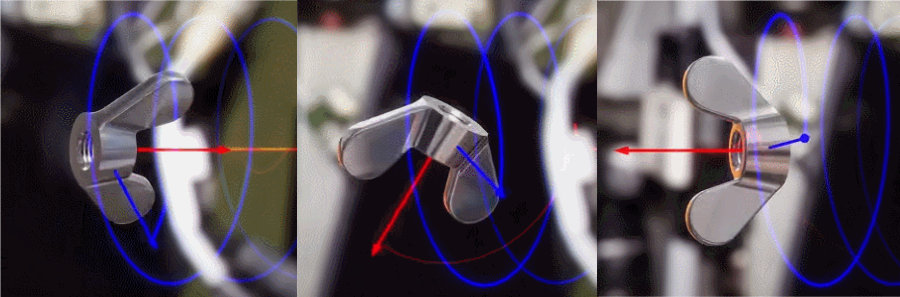
\includegraphics[width=0.9\textwidth]{dzhani.jpg}
\end{center}
   \caption{Eine Darstellung des Dzhanibekov-Effekts \cite{28}.}
\label{fig:10}
\end{figure*}

Das Prinzip hinter einer schnellen Änderung der Erdrotationsachse liegt in der Physik rotierender Objekte. Das kanonische Beispiel dafür ist der Dzhanibekov-Effekt, entdeckt vom russischen Astronauten Vladimir Dzhanibekov \cite{37}, und dargestellt in Abbildung \ref{fig:10}. Ein Objekt, das nicht perfekt um eine seiner drei Hauptträgheitsachsen rotiert, wird keine feste Rotationsachse beibehalten. Wenn es nahe seiner zweiten Hauptachse rotiert, wird es scheinbar plötzlich auftretende Rotationswechsel durchmachen. Auch wenn dies nicht genau das ist, was wir glauben, während der schnellen Umkehrungen der Erde geschieht, ist der Punkt, dass in Abwesenheit äußerer Kräfte nur die Rotationsphysik eine schnelle Änderung der Rotationsachse der Erde erklären kann.

Um genau zu sein, erfährt die Erde höchstwahrscheinlich keinen einfachen und gleichmäßigen Dzhanibekov-Effekt. Wäre dies der Fall, wären wir in der Lage, eine allmähliche Verschiebung der Erdrotationsachse im Laufe der Zeit zu erkennen. Vielmehr glauben wir, dass die Erde periodische, plötzliche Störungen in ihrer physischen Struktur erfährt, die zu einer Entkopplung ihrer "äußeren Rotationskörper" (Kruste/Mantel) und "inneren Rotationskörper" (Kern) führen. Ohne eine externe Eingabe besagt das Gesetz der Erhaltung des Drehimpulses, dass die Erde ihre Rotationsachse nicht plötzlich ändern kann; daher ist eine Entkopplung der äußeren und inneren Rotationskörper eine der wenigen Möglichkeiten, abgesehen von einem externen Aufprall auf die Erde, die eine plötzliche und abrupte Umkehr verursachen könnten.
Der spezifische Prozess, der die interne Störung der Erde antreibt, wird für einen Zustandswechsel in der Struktur von Eisen gehalten, das den Kern der Erde bildet (Abbildung \ref{fig:11}). Der innere Kern besteht aus hexagonal dichtgepacktem Eisen (Fe) \cite{141}. Wenn dieses hcp-Fe in einen flüssigen metallischen Zustand umgewandelt wird, setzt es kinetische Energie frei und wird in den äußeren Kern abgeschüttet. Dieser Phasenwechsel verringert die magnetische Permeabilität des Kerns, schwächt das geomagnetische Feld und setzt Wärme frei, wodurch LLVP-Strukturen (große Scherprovinzen mit geringer Geschwindigkeit) (Abbildung \ref{fig:12}) \cite{38} im Mantel entstehen und die Erdoberfläche über die abyssalischen Ozeane erwärmt wird. Beide Trends sind in den letzten Jahrhunderten gut dokumentiert worden und werden später in diesem Dokument erörtert.

\begin{figure*}[t]
\begin{center}
\includegraphics[width=1\textwidth]{layers.jpg}
\end{center}
   \caption{Darstellung der inneren Erdprozesse, die zum ECDO-Flips führen \cite{129}.}
\label{fig:11}
\end{figure*}

\begin{figure}[t]
\begin{center}
   \includegraphics[width=1\linewidth]{llvp.jpg}
\end{center}
   \caption{Eine detaillierte Darstellung des LLVP unter Südafrika \cite{28}.}
\label{fig:12}
\label{fig:onecol}
\end{figure}

Es wird angenommen, dass derselbe Prozess im Inneren der Erde, rückwärts ablaufend, auch die Rückkehr in den aktuellen Rotationszustand der Erde relativ bald nach dem Flip antreibt.

\section{Beweise für einen bevorstehenden Erden-Flip}

Es gibt starke Gründe zu der Annahme, dass wir kurz vor einem weiteren Erden-Flip stehen. Ein Kataklysmus ist seit mehreren Jahrtausenden nicht aufgetreten, was ungefähr der Häufigkeit entspricht, mit der diese Ereignisse basierend auf historischen Berichten und Daten zu geschehen scheinen. Die stärksten Daten, die einen bevorstehenden Flip unterstützen, stammen aus jüngsten geomagnetischen Daten, die darauf hindeuten, dass das magnetische Feld der Erde seit ungefähr zweitausend Jahren schwächer wird. Diese Abschwächung hat sich beschleunigt und in den letzten Jahrzehnten alarmierende Raten erreicht.

In Abbildung \ref{fig:14} ist das geomagnetische Feld der Erde in den Jahren 1590 und 2025 dargestellt \cite{125,126}. Wie in der Abbildung gezeigt, hat sich das Feld erheblich abgeschwächt.

Ein weiteres Maß für das schwächer werdende geomagnetische Feld ist die Position des geomagnetischen Nordpols (Abbildung \ref{fig:13}). Der geomagnetische Norden befand sich historisch im kanadischen Arktisgebiet. Er ist jedoch in den letzten Jahrhunderten langsam gewandert und hat sich vor wenigen Jahrzehnten erheblich beschleunigt. Er bewegt sich jetzt mit einer Geschwindigkeit von 55 Kilometern pro Jahr rasch in Richtung Russland \cite{124}.

\begin{figure*}[t]
\begin{center}
\includegraphics[width=0.9\textwidth]{saa.jpg}
\end{center}
   \caption{Eine Darstellung des schwächer werdenden geomagnetischen Feldes von 1590 bis 2025. Berechnet mit den Modellen gufm1 und IGRF-14 \cite{125,126}.}
\label{fig:14}
\end{figure*}

\begin{figure}[t]
\begin{center}
   \includegraphics[width=1\linewidth]{npw.jpg}
\end{center}
   \caption{Die Position des geomagnetischen Nordpols von 1590 bis 2025, in 5-Jahres-Schritten dargestellt \cite{142}.}
\label{fig:13}
\label{fig:onecol}
\end{figure}

\begin{figure}[t]
\begin{center}
   \includegraphics[width=1\linewidth]{ocean-highlight.jpg}
\end{center}
   \caption{Erwärmungsraten von tiefen (>$2000\,\text{m}$ Tiefe) Ozeanen von 1991 bis 2010, in Rot eingekreist \cite{132}.}
\label{fig:15}
\label{fig:onecol}
\end{figure}

Es wird angenommen, dass das Magnetfeld der Erde von einem inneren Dynamo erzeugt wird - kreisförmige Säulen von Magmaströmungen, die sich aufgrund der Rotation im äußeren Erdkern bewegen \cite{123}. Ein schwächer werdendes geomagnetisches Feld ist ein Anzeichen für Störungen tief im Inneren der Erde. Nach der ECDO-Theorie stoßen diese Störungen Wärme aus und führen schließlich zur Entkoppelung des Mantels und des Kerns, was zu einem Erden-Flip führt \cite{1}.

Es gibt beträchtliche Daten, die die Anwesenheit exothermer Prozesse im Erdinneren bestätigen. Eine Erwärmung der Erde ist dokumentiert durch steigende kontinentale und ozeanische Oberflächentemperaturen \cite{127,128}, steigende atmosphärische CO2-Werte, die im Einklang mit den Wärmeplumes der Erde steigen \cite{129,130}, und eine Abnahme der globalen Meereis-Ausdehnung \cite{131}. Die Daten legen nahe, dass steigende CO2-Werte und Temperaturen nicht die Ursache des „menschengemachten“ Klimawandels sind, sondern Folgeerscheinungen eines exothermen Kerns \cite{129}.

Am bedeutendsten zeigen Studien zu Erwärmungsraten in der Tiefsee (Tiefe $>$2000 Meter), dass nicht nur die Tiefsee erwärmt wird, sondern die stärksten Erwärmungsraten in der abyssalen Schicht (4000 - 6000 m) zu finden sind. Diese Tiefseeerwärmung hat einen Schwerpunkt unterhalb von 4000 Metern \cite{132,129}, was nicht möglich wäre, wenn die Ozeane von oben durch die Atmosphäre erwärmt würden. Solche Daten liefern starke Unterstützung für die These, dass die jüngsten Klima- und geomagnetischen Veränderungen von Prozessen tief im Inneren der Erde angetrieben werden. Abbildung \ref{fig:15} zeigt die globalen Erwärmungsraten der Tiefsee von 1991 bis 2010 \cite{132}.

\section{Modellierung der bevorstehenden Erdachsendrehung}

\begin{figure}[b]
\begin{center}
   \includegraphics[width=1\linewidth]{saa-crop.jpeg}
\end{center}
   \caption{Eine Berechnung des Kipppunkts basierend auf der südlichen atlantischen Anomalie weist auf ein Datum vom 13. März 2059 hin \cite{125,126}.}
\label{fig:16}
\label{fig:onecol}
\end{figure}

Die Vorhersage des Zeitpunkts der nächsten Erdachsendrehung ist eine komplexe Aufgabe. Derzeit liegt das beste Modell dafür im geomagnetischen Feld der Erde - der südlichen atlantischen Anomalie (SAA). Diese Region über dem Südatlantik hat die schwächste geomagnetische Feldstärke und ist definiert als der Bereich mit einer Feldstärke unter 32.000 Nanotesla \cite{135}, was der schwächste Feldwert im Jahr 1590 war. Die Oberfläche der südlichen atlantischen Anomalie hat sich von 1 % der Erdoberfläche im Jahr 1590 auf 21 % im Jahr 2025 vergrößert \cite{136}.

Um eine Schätzung dafür zu erhalten, wann sich die Erde drehen könnte, habe ich die Daten zur Ausdehnung der SAA-Oberfläche an eine Potenzgesetz-Kipppunkt-Gleichung angepasst, die ein komplexes System modelliert, das sich einem kritischen Übergang nähert, bei dem das System eine dramatische und abrupte Änderung erfährt. Meine Berechnungen ergaben einen vorhergesagten Kipppunkt am 13. März 2059 (Abbildung \ref{fig:16}). Diese Vorhersage würde umso genauer werden, je näher wir dem Übergang kommen \cite{136}.

Andere Metriken wie das Wandern der Rotationsachse, Wetteranomalien sowie seismische und vulkanische Daten können ebenfalls helfen, eine bessere Vorhersage darüber zu treffen, wann die nächste Erdachsendrehung stattfinden könnte.

\section{Historische Zeitleiste der ECDO}

Während es schwierig ist, eine genaue Zeitleiste für vergangene ECDO-Ereignisse zu erstellen, scheint es, dass es mindestens 2 ECDO-Ereignisse während des Holozäns gab. Beachten Sie den Bericht, den Herodot von ägyptischen Priestern erzählte, dass \textit{"vom ersten König bis zu diesem Priester von Hephaistos, der zuletzt regierte, es dreihunderteinundvierzig Generationen von Menschen gegeben hatte... In dieser Zeit sagten sie, dass die Sonne viermal von ihrem üblichen Aufgangspunkt verschoben wurde, und dort, wo sie jetzt untergeht, hatte sie zweimal ihren Aufgang, und an dem Ort, von dem aus sie jetzt aufgeht, hatte sie zweimal ihren Untergang"} \cite{32}. Platon, der im fünften Jahrhundert v. Chr. lebte \cite{111}, erklärte, dass nach der Flut, die Atlantis in einem einzigen Tag und einer Nacht 9.000 Jahre zuvor ertränkte, \textit{"es seitdem viele Überschwemmungen gegeben hat und die Überlebenden in den Bergen die Kunst des Schreibens nicht kannten und sich über viele Generationen hinweg ausschließlich darauf konzentrierten, die Mittel zum Leben zu erwerben"} \cite{112}, was darauf hindeutet, dass es seit dem Ende der Jüngeren Dryas etwa 9700 v. Chr. mehr als zwei Achsendrehungen gab. Die physischen Beweise, die in diesem Artikel und in meiner Forschung \cite{2} behandelt werden, liefern reichlich Beweise für Platons Bericht.

Der jüngste Kandidatentermin für eine ECDO-Umkehr liegt in der Zeit von 2300 bis 1600 v. Chr., auf die viele katastrophale Flutberichte (Gun-Yu \cite{113,114,115}, Ogyges \cite{116,117}, Peru \cite{118,119}, Exodus \cite{120}), zivilisatorische Zerstörungen und Leerstände (Mohenjo-Daro \cite{121}, minoisches Kreta\cite{100,101}) und physikalische Anomalien (Bond-Ereignisse \cite{122}, 4,2 Kilo-Jahr-Ereignis \cite{90}) datiert wurden. Es gibt keine umfangreiche Beweiskonvergenz jüngeren Datums, die auf ein großes katastrophales Ereignis hindeutet.

\section{Schlussfolgerung}

Operation NANOOK war ein Aufklärungseinsatz der Vereinigten Staaten während des Kalten Krieges zur Kartierung der Arktis und der nördlichen Sowjetküste nach dem Zweiten Weltkrieg \cite{137}. Während ihrer Untersuchung stellten sie fest, dass der magnetische Pol 125 bis 200 Meilen nördlich von dem lag, wo er laut den Ergebnissen früherer Expeditionen sein sollte. Dementsprechend \textit{"stellte sich unter den Regierungswissenschaftlern die Frage, was passieren würde, wenn die magnetischen und geografischen Pole zusammenfielen. Um dies zu beantworten, wurde die Rand Corporation unter der Projektleitung von Dr. Paul A. Siple damit beauftragt, Laborstudien mit Modellen der Erde durchzuführen, die aus konzentrischen Kugeln bestanden – einer inneren Kugel, die den elektromagnetisch geladenen, geschmolzenen Eisenkern der Erde darstellte, dessen Achse die „magnetischen“ Pole definierte; und einer äußeren Kugel, die die Erdkruste darstellte, die sich um eine „geografische“ Polachse drehte. Durch wiederholte Experimente wurde festgestellt, dass der „magnetische“ Pol, wenn er sich dem „geografischen“ Pol nähert, seine Konvergenzgeschwindigkeit an einem bestimmten Punkt zu beschleunigen scheint, als würde er durch Zentripetalkraft zum „geografischen“ Pol hingezogen, und mit diesem zusammenfällt. Stattdessen würde der „magnetische“ Pol jedoch schnell um den „geografischen“ Pol „flippen“, dann wie durch Zentrifugalkraft angezogen, sich in Richtung Äquator drehen und schließlich an einer Position enden, bei der die beiden Achsen eine ungefähre Divergenz von 89 Grad annehmen. Nachdem dieser Pol-„Flip“ aufgetreten ist, würden die Achsen dann allmählich beginnen, sich im Laufe einer langen Zeit wieder zu konvergieren"} \cite{138,139}.

Anschließend \textit{"diskutierten die Wissenschaftler bei einem der wissenschaftlichen Treffen, die Major White Anfang 1948 im Pentagon besuchte, über die Klugheit, die Öffentlichkeit über das bevorstehende Polflip-Phänomen zu informieren. Keiner der Wissenschaftler wollte die Information vor der Öffentlichkeit zurückhalten; andererseits konnten sie sich auch nicht darauf einigen, wie sie veröffentlicht werden sollte. Das Wissen um dieses Phänomen, so fühlten einige, könnte an und für sich das moralische Gefüge der Gesellschaft zerstören. Ihre Befürchtungen erwiesen sich offenbar als unbegründet, als in den frühen 1950er Jahren Informationen über das Flip-Phänomen sowohl in einer Zeitungskolumne als auch in einem Zeitschriftenartikel veröffentlicht wurden, was jedoch überraschenderweise keine Reaktionen von einer offenbar verblüfften, provinziellen oder ungläubigen Öffentlichkeit hervorrief"} \cite{138,139}.

Warum schenken wir dem keine Beachtung? Es gibt reichlich Grund zu der Annahme, dass die Erde bereits umgekippt ist. Dieses Papier bietet zusammen mit dem zweiten Teil des Papiers eine dichte Zusammenfassung einer großen Konvergenz von Beweisen aus vielen Bereichen, die darauf hindeuten, dass dies der Fall ist, wie etwa Flutgeschichten aus der ganzen Welt, Salz- und Meeresfossilien, die die Kontinente bedecken, alte unterirdische Schutzräume, Tierüberreste und katastrophale geologische Landschaften. Der Mensch soll angeblich Hunderttausende von Jahren alt sein, doch die moderne Geschichte reicht nur einige tausend Jahre zurück. Könnte es nicht sein, dass die Erde in regelmäßigen Abständen kippt, die Kontinente sauber gewischt werden und wir gezwungen sind, wieder bei null anzufangen – in der Steinzeit –, wodurch unsere Aufzeichnungen der alten Geschichte auf eine Handvoll katastrophaler Geschichten reduziert werden? Wenn dem so ist, könnte die Verhinderung, dass dies erneut geschieht, eine der wichtigsten Aufgaben der Menschheit sein.
Abschließend möchte ich Ihnen diesen Bericht aus dem Timaeus, geschrieben von Platon, über ein Gespräch zwischen Solon, einem athenischen Staatsmann, und ägyptischen Priestern hinterlassen \cite{140}: \textit{"Und bei einer Gelegenheit, als [Solon] sie dazu verleiten wollte, über die alte Geschichte zu sprechen, versuchte er, ihnen die älteste unserer Überlieferungen zu erzählen, über Phoroneus, der als der erste Mensch galt, und Niobe; und er fuhr fort, die Legende über Deukalion und Pyrrha nach der Flut zu erzählen und wie sie sie überlebten und die Genealogie ihrer Nachkommen anzugeben; und indem er die Anzahl der Jahre berechnete, die die erwähnten Ereignisse einnahmen, versuchte er, die Zeiträume zu berechnen. Daraufhin sagte einer der Priester, ein ungemein alter Mann: „O Solon, Solon, ihr Griechen seid immer Kinder: Es gibt nicht so etwas wie einen alten Griechen“. Und als er dies hörte, fragte er: „Was meinst du mit diesem Spruch?“ Und der Priester antwortete: „Ihr seid alle jung in der Seele. Denn ihr habt darin keinen einzigen Glauben, der alt und aus alter Überlieferung stammt, noch eine Wissenschaft, die mit Alter ehrwürdig ist. Und dies ist der Grund dafür: Es hat viele und verschiedene Zerstörungen der Menschheit gegeben und wird es geben, von denen die größten durch Feuer und Wasser und die kleineren durch unzählige andere Mittel verursacht werden. Denn wahrlich, die Geschichte, die in eurem Land ebenso erzählt wird wie in unserem, wie einstmals Phaethon, der Sohn des Helios, den Wagen seines Vaters spannte und, weil er ihn nicht auf dem von seinem Vater genommenen Kurs lenken konnte, alles auf der Erde verbrannte und selbst durch einen Blitz umkam - diese Geschichte hat, wie sie erzählt wird, die Form einer Legende, doch die Wahrheit davon liegt in der Verschiebung der Körper am Himmel, die um die Erde kreisen, und in einer Zerstörung der Dinge auf der Erde durch heftiges Feuer, das in langen Abständen wiederkehrt. Zu solchen Zeiten leiden alle, die auf den Bergen und an hohen und trockenen Orten wohnen, mehr Zerstörung als diejenigen, die in der Nähe von Flüssen oder dem Meer wohnen; und in unserem Fall bewahrt uns der Nil, unser Erlöser auf andere Weise, auch in solchen Zeiten vor dieser Katastrophe, indem er hoch steigt. Und wenn andererseits die Götter die Erde mit einer Flut von Wasser reinigen, werden alle Hirten und Schäfer, die in den Bergen sind, gerettet, aber die in den Städten eures Landes werden von den Strömen ins Meer gespült; wohingegen in unserem Land das Wasser weder damals noch zu irgendeiner anderen Zeit über unsere Felder von oben herunterströmt, im Gegenteil, es neigt dazu, sich von unten nach oben zu erheben. Daher wird hier das, was aufbewahrt wird, als das älteste betrachtet; die Wahrheit ist, dass an jedem Ort, wo keine übermäßige Hitze oder Kälte es verhindert, immer irgendeine menschliche Bevölkerung existiert, mal mehr, mal weniger zahlreich. Und wenn ein Ereignis stattgefunden hat, das edel oder groß oder in irgendeiner Weise auffällig ist, sei es in eurem Land oder in unserem oder an einem anderen Ort, von dem wir durch Bericht wissen, all solche Ereignisse werden seit jeher aufgezeichnet und hier in unseren Tempeln aufbewahrt; während eure Leute und die anderen jedes Mal nur mit Schriftzeichen und all solch eine Künste ausgestattet sind, die zivilisierte Staaten benötigen, und wenn nach dem üblichen Zeitabstand, wie eine Plage, die Flut des Himmels aufs Neue über euer Volk hereinbricht, bleibt keiner von euch übrig, außer den ungebildeten und ungeschulten, sodass ihr so jung wie immer werdet, ohne Kenntnis all dessen, was in alten Zeiten in diesem Land oder in eurem eigenen geschehen ist. Gewiss, die Genealogien, die du gerade eben erzählt hast, Solon, die das Volk deines Landes betreffen, sind kaum besser als Kindergeschichten; denn erstens erinnert ihr euch nur an eine Flut, obwohl viele zuvor stattgefunden haben; und zweitens seid ihr unwissend darüber, dass das edelste und vollkommenste Geschlecht unter den Menschen in dem Land geboren wurde, in dem ihr jetzt wohnt, und von ihnen stammen sowohl du selbst als auch die gesamte bestehende Stadt, aus einem kleinen Samen, das zufällig übrig blieb; aber dies ist dir entgangen, weil über viele Generationen die Überlebenden starben, ohne die Möglichkeit, sich schriftlich auszudrücken. Denn wahrlich, zu einer Zeit, Solon, vor der größten Zerstörung durch Wasser, war der heutige athenische Staat der tapferste im Krieg und auch in jeder anderen Hinsicht überaus gut organisiert. Es wird gesagt, dass es die prächtigsten Kunstwerke und die edelste Staatsform jeder Nation unter dem Himmel besaß, von der wir erzählt bekommen haben”}.

Diese Priester erzählten Solon natürlich auch von der alten Zivilisation von Atlantis: \textit{"Denn alles, was wir hier haben, das innerhalb des Mundes liegt, von dem wir sprechen, ist offensichtlich ein Hafen mit einem schmalen Eingang; aber dort drüben ist ein echtes Meer, und das Land, das es umgibt, kann in der vollsten und wahrsten Bedeutung am allermeisten ein Kontinent genannt werden. Nun existierte auf dieser Insel Atlantis eine Konföderation von Königen von großer und wunderbarer Macht, die über die ganze Insel und über viele andere Inseln und Teile des Kontinents herrschten; und darüber hinaus herrschten sie über die Länder hier innerhalb der Meerenge Libyen bis nach Ägypten und über Europa bis nach Tyrrhenien. Also versuchte dieses Heer, als es sich vollständig versammelt hatte, einmal bei einem einzigen Angriff sowohl euer Land als auch unseres und das ganze Gebiet innerhalb der Meerenge zu versklaven. Und dann war es, Solon, dass die Männlichkeit eures Staates sich für Tapferkeit und Macht in den Augen der ganzen Welt herausragend zeigte. Denn es stand in Tapferkeit und allen kriegerischen Künsten über allen, und indem es teils als Führer der Griechen agierte, teils allein und verlassen von allen anderen, nachdem es die tödlichsten Gefahren durchgemacht hatte, die Eindringlinge besiegte und eine Trophäe errichtete; wodurch es vor der Sklaverei solche rettete, die noch nicht versklavt waren, und den Rest von uns, die innerhalb der Grenzen des Herakles wohnen, frei machte. Aber später ereigneten sich schreckliche Erdbeben und Überschwemmungen, und ein schwerer Tag und eine Nacht ereilten sie, als der gesamte Körper eurer Krieger von der Erde verschluckt wurde und die Insel Atlantis ebenso vom Meer verschlungen wurde und verschwand"}.

\section{Danksagungen}

Danke an Ethical Skeptic, den ursprünglichen Autor der ECDO-Abhandlung, dafür, dass er seine aufschlussreiche, bahnbrechende Abhandlung abgeschlossen und mit der Welt geteilt hat. Seine dreiteilige Abhandlung \cite{1} bleibt das grundlegende Werk zur Theorie der exothermen Kern-Mantel-Entkoppelung Dzhanibekov-Oszillation (ECDO) und enthält weit mehr Informationen zu diesem Thema, als ich hier kurz behandelt habe.

Danke an Ankit, der die Katastrophen-Kompilationsdaten in Tabelle 1 verarbeitet hat.

Und natürlich danke an die Giganten, auf deren Schultern wir stehen; diejenigen, die all die Forschung und Untersuchung betrieben haben, die diese Arbeit möglich gemacht haben und daran gearbeitet haben, Licht für die Menschheit zu bringen.

\clearpage
\twocolumn

\section{Zusätzliche Bilder}

\begin{figure}[H]
\begin{center}
   \includegraphics[width=1\linewidth]{wave.jpg}
\end{center}
   \caption{Ein genauer Blick auf die unterhöhlte, parabolische Wellenerosion an der Chephren-Pyramide \cite{27}.}
\label{fig:19}
\label{fig:onecol}
\end{figure}

\begin{figure}[H]
\begin{center}
   \includegraphics[width=1\linewidth]{star-stone.jpg}
\end{center}
   \caption{Die Sternkarte, die in einen der Schächte der Cheops-Pyramide eingraviert ist \cite{28}.}
\label{fig:20}
\label{fig:onecol}
\end{figure}

\begin{figure*}[t]
\begin{center}
\includegraphics[width=1\textwidth]{deepsea.jpg}
\end{center}
   \caption{Eine visuelle Darstellung der Tief- und Abyssal-Meerheizungsanomalie im Vergleich zu einer normalen atmosphärischen Meerheizungskurve. Die gesamte Heizungsanomalie wurde von NOAA entnommen \cite{147}, die Verteilungen der Tief- und Abyssalheizung aus einer Studie von Desbruyeres \cite{132} und die Datenverarbeitung und Visualisierung von Ethical Skeptic \cite{129}.}
\label{fig:21}
\end{figure*}

\begin{figure*}[t]
\begin{center}
\includegraphics[width=1\textwidth]{sealevel.jpeg}
\end{center}
   \caption{Der Meeresspiegel zeigt über 75 Jahre hinweg eine 20\%ige Zunahme der Varianz über 63 Stationen, was auf eine Erhöhung der Strömungsgeschwindigkeit hindeutet. Anstiege in der Meeresspiegelvarianz treten gleichzeitig mit ozeanischen Wärmepulsen auf, was darauf hindeutet, dass diese beide durch Erhitzung von tief unter den Ozeanen der Erde verursacht werden könnten \cite{2,129}.}
\label{fig:22}
\end{figure*}
\begin{figure*}[t]
\begin{center}
\includegraphics[width=1\textwidth]{co2.jpg}
\end{center}
   \caption{Atmosphärisches CO2 ppm ist in den letzten 45 Jahren stetig gestiegen, wahrscheinlich verursacht durch einen Anstieg der Meerestemperaturen. Quelle: NOAA \cite{148,129}.}
\label{fig:23}
\end{figure*}

\begin{figure*}[t]
\begin{center}
\includegraphics[width=1\textwidth]{ice.jpg}
\end{center}
   \caption{Die weltweite Meereisausdehnung ist in den letzten 45 Jahren zurückgegangen, aufgrund einer Erwärmung der Erde. Quelle: ADS \cite{149}.}
\label{fig:24}
\end{figure*}

\clearpage
\twocolumn

{\small
\bibliographystyle{ieee}
\bibliography{egbib}
}

\end{document}
